\section{Analisi}

\begin{wrapfigure}{r}{50mm}
    \vspace{-10mm}
    \begin{center}
        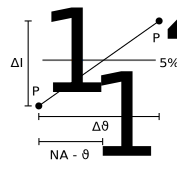
\includegraphics[width=48mm]{drawing.pdf}
    \end{center}
    \vspace{-10mm}
\end{wrapfigure}

Poiché abbiamo misurato tre valori distinti di intensità massima $I\ped{max}$ e $\vartheta\ped{max}$, occorre innanzitutto ricavarne un unico valore. Abbiamo quindi fatto la media dei valori registrati. Dopo questo primo passo ci siamo assicurati di esprimere tutti gli angoli rispetto
all'angolo $\vartheta\ped{max}$, ovvero lo abbiamo sottratto a tutti gli altri angoli.

Abbiamo graficato i dati, ottenendo lo spettacolare grafico in Figura \ref{fig:graph}, tracciando una linea orrizzontale
che corrisponde al 5\% dell'intensità massima. Chiaramente la curva interseca due volte la linea del 5\%, poiché è simmetrica.
Si possono quindi trovare due valori diversi di apertura numerica, e noi li abbiamo calcolati entrambi, come segue.
Dal grafico abbiamo trovato i punti tra i quali passa la linea corrispondente al 5\%,
che indicheremo con $P_1$, $P_2$ rispettivamente. $I_1$, $I_2$ e $\vartheta_1$, $\vartheta_2$ indicano rispettivamente le intensità e gli angoli
relativi ai due punti. Quindi si può ottenere il valore di \emph{NA} interpolando linermente tra i due punti e imponendo:

\begin{equation}
        0.05 \cdot I\ped{max} = I_1 + (I_2 - I_1) \cdot \frac{\emph{NA} - \vartheta_1}{\vartheta_2 - \vartheta_1} \\
                              = I_1 + \Delta I \cdot \frac{\emph{NA} - \vartheta_1}{\Delta \vartheta}
\end{equation}

Da cui si ha, banalmente:

\begin{equation}
    \emph{NA} = \frac{\Delta \vartheta}{\Delta I} (0.05 \cdot I\ped{max} - I_1) + \vartheta_1
\end{equation}

I valori che noi abbiamo calcolato risultano compatibili e sono i seguenti:

\begin{equation}
    \emph{NA}_1 = 0.505 \pm 0.01 \qquad \emph{NA}_2 = -0.5033 \pm 0.007
\end{equation}